Des données transmisent en utilisant le protocole IPv4 sont encapsulées dans un message que
l'on appelle un paquet IPv4. Ces paquets sont constitués d'un entête suivis des données à transmettre.

% Mossi
\subsection{Adresse IPv4}

L'entête contient des informations essentielles pour la transmission d'un paquet, notamment les
adresses source et destination.

Une adresse IP sert à identifier une machine (et plus précisément une des interfaces de cette machine)
dans un réseau particulier.
Comme nous le verrons plus tard cet identifiant unique permet de désigner à la fois un
réseau et une machine précise au sein de ce réseau.
Une adresse est codé sur 32 bits ce qui permet de coder 2\^32 soit 4294967296 adresses différentes.
Par convention on peut représenter une adresse IPv4 comme une suite de 4 nombres décimaux séparés par des points,
chacun traduisant un octet. Cette représentation a contribué à simplifier l'utilisation et la manipulation
des adresses.
Comme chaque nombre représente un octet, les valeurs de celui-ci sont comprises entre 0 et 255.

\vspace{1cm}
Exemple: adresse à valeur décimale: 212.217.0.1 => correspond sous sa forme
binaire à: 11010100.11011001.00000000.00000001
\vspace{1cm}

\subsubsection{Notion de NET ID et HOST ID}
Une adresse IPv4, en tant qu'identifiant d'une machine dans un réseau, contient deux informations:
une première partie qui identifie le réseau appelé NET ID (les bits de poids fort), une seconde qui identifie l’hôte appeler host-ID (les bits de poids faible).
Les machines qui se trouvent donc sur le même réseau partage le même NET ID pour leur adresse.

La longueur de ces deux parties est variable: la taille du HOST ID dépend de la taille du NET ID. Pour représenter la longueur de ces différentes parties on a introduit la notion de masque

\subsubsection{Masque de réseau}

Le masque sert à représenter la scission entre le NET ID et le HOST ID.
Il est codé sur 32 bits et adopte la même représentation qu'une adresse IP, à savoir
4 nombres décimaux séparé par des points.
La position des bits à 1 dans le masque corresponde à la position des bits définissant le NET ID dans l'adresse IP.
Pour obtenir les bits du NET ID il suffit de faire un ET logique entre l'adresse et son masque. Tous les autres bits (donc les bits à 0)
feront donc partie du HOST ID.
Les bits à 1 sont contiguës et commencent au bit de poids fort: le nombre de bit à 1 dans le masque, donne
le nombre de bit faisant partie du NET ID en partant du bit de poids fort dans l'adresse.

En conséquence plus le nombre de bit à 1 dans le masque est grand, plus le NET ID sera grand, et plus le HOST ID sera petit, car il restera moins de bit pour définir le HOST ID (la somme des deux devant évidemment faire 32 bits).

\begin{center}
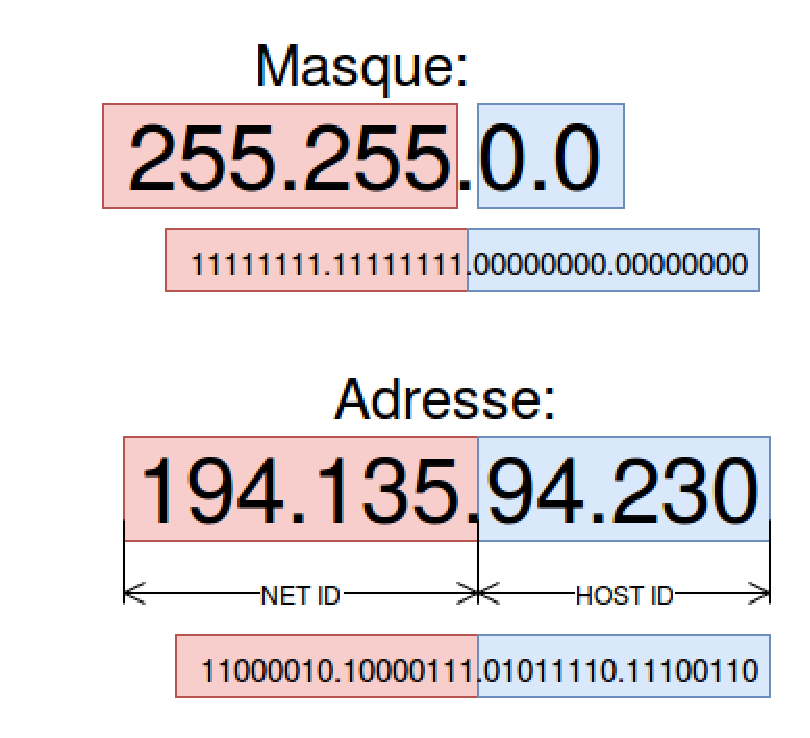
\includegraphics[width=7cm]{./pics/maskipv4.eps}
\end{center}

//TODO exemple
//TODO exemple invalide

\subsubsection{Classes d'adresse IP}
Historiquement les classes d'adresse IP correspondaient à une plages d'adresses avec un masque figer pour une classe donnée.
Ce système permettait de déduire le masque en fonction
de l'adresse IP étant donné que chaque classe avait son masque défini de manière standard.
Il fut décrit dans le RFC 791\cite{url-RFC-791}.

//TODO tableau classe

A partir de ce tableau nous pouvons voir qu'il suffit de regarder les 4 bits de
poids fort pour déduire à quelle classe appartient une adresse.  Par exemple si
une machine à pour adresse 152.123.87.45 on sait en regardant les 4 premiers
bits que cette adresse fait partie de la classe B (car l'adresse commence par
10). De là, la machine n'a pas besoin de masque en plus car elle sait que le
masque correspondant un adresse de classe B est 255.255.0.0 .

Ce système permet donc d'adresser de nombreux réseaux avec un nombre de machine
variable en fonction de la classe, et tout cela sans avoir besoin de
communiquer ou de paramétrer un masque; celui-ci étant normalisé pour chaque
classe.  Cependant il a un gros inconvénient, étant donné que les masques sont
figé, un réseau peux ne peux pas utiliser une partie plus ou moins importante
de ses adresses. Par exemple si un réseau contient 500 machines, il ne peux pas
utiliser d'adresse de classe A étant donné que celle-ci ne permettent d'avoir
que des réseaux de 254 machines maximum. Il va donc falloir utiliser des
adresses de classe B minimum, car elles permettent d'adresser 65534 machines au
sein d'un réseau. Nous pouvons donc utiliser 500 adresses sur les 65534
disponible, mais le reste sera "perdu".  Ce système était simpliste mais
n'était pas utilisable sur le long terme car il "gâche" des adresses en
n'utilisant pas tout son espace d'adressage.


\subsubsection{CIDR}

Aujourd'hui le système le plus utilisé est CIDR (Classless Inter-Domain
Routing) remplace le système de classe d'adresse. CIDR permet de créer des
masque beaucoup plus fin, étant donné qu'on n'est plus limité à des masque de
réseau fixe, on peut ajuster le masque pour avoir le nombre de machine
adressable dans un réseau le plus proche possible du nombre de machine que l'on
souhaite adressé.  Cela permet de limiter les pertes en adresse inutilisé, si
la plage est correctement découpée.  On peut donc créer des masques à la
séparation entre le NET ID et le HOST ID se trouve n'importe où, même en plein
milieu des octets (ce qui était impossible avec les classes d'adresse), ce qui
apporte une plus grande flexibilité.  Cela permet aussi de créer une hiérarchie
dans une plage d'adresse réseau qui serait découper en plusieurs réseaux
"fils", et cela permet notamment, avec cette hiérarchie, de réduire la table de
routage des routeur.  De là est né une nouvelle notation des masques: on écrit
le nombre de bit à 1 dans le masque à la suite de l'adresse IP et séparé par un
slash.


\begin{center}
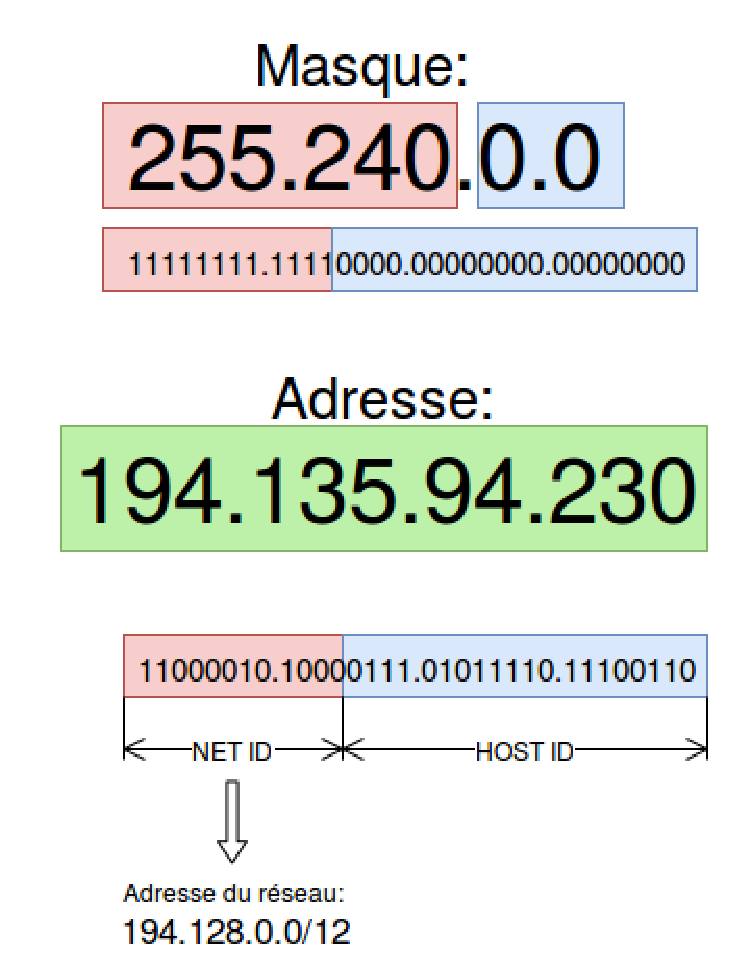
\includegraphics[width=7cm]{./pics/maskipv4cidr.eps}
\end{center}



\subsubsection{Types d'adresses}
La variété des exigences en matière de réseaux a donnée lieu à une
classification progressive des adresses selon des rôles bien précis. En effet,
pas toutes les adresses IPv4 ont la même signification: à certaines adresses
(ou plages d'adresses) ont été attribué par convention des fonctions ou des
caractéristiques particulières.  Dans la suite de cette partie nous analyserons les
adresses IP sous trois aspects différents: nous classifierons d'abord les adresses selon
le type de diffusion qu'elles permettent d'effectuer, puis nous introduirons le
concept d'adresse publique et d'adresse privée, enfin nous parlerons de l'utilisation
particulière qui a été faite avec certaines adresses.



\paragraph{Mode de diffusion}
Dans le cadre des transmissions, en plus de communiquer entre deux interfaces, il est 
parfois nécessaire qu'un message soit reçu par un groupe de machines ou que 
même la totalité du réseau reçoivent ce message.

On a défini pour cela plusieurs types de diffusions associés à certaines adresses particulières.

Le type de diffusion le plus utilisé est la diffusion en unicast. Dans ce mode,
l'adresse IP désigne une machine de manière unique. L'adresse IP appartient
à une seule machine et sert à l'identifier sur un réseau.  C'est le type
d'adresse que nous avons abordé jusqu'à présent.  Mais il peut être intéressant
de pouvoir contacter plusieurs machines en même temps. On pourrait bien sûr
envoyer des paquets en unicast à chaque machine que l'on souhaite contacter,
mais cela serait fastidieux et inonderait le réseau inutilement. Une solution plus
pratique est d'avoir une adresse qui désigne plusieurs machines à la fois. Cela
permet d'envoyer un seul paquet qui est remis à plusieurs machines. Il
existe pour faire cela plusieurs types de diffusion.
\begin{itemize}
\item Le broadcast: Ce mode de diffusion permet d'envoyer un paquet unique tout en 
joignant toutes les machines sur un réseau. Lorsque les machines reçoivent ce
paquet, elles s'aperçoivent que l'adresse de destination du paquet est l'adresse de
broadcast et elles vont alors traiter le paquet. L'adresse de broadcast d'un réseau
est défini comme la plus "haute" adresse du réseau: cela se traduit par la mise
à 1 de tous les bits de la partie HOST ID. Cette adresse ne peut donc pas être
attribuée à une machine en tant qu'adresse unicast.  Le broadcast est utilisé
par des protocoles tel que ARP et DHCP.  Nous pouvons remarquer qu'avec cette
définition, nous pouvons envoyer un message de broadcast à n'importe quel
réseau, incluant le notre. En réalité (sauf
configuration volontaire) les routeurs ne laissent pas passer les messages de
broadcast d'un réseau à un autre; excepté quelques cas spéciaux comme DHCP où un
serveur peut s'adresser à plusieurs réseaux, et où ses messages de broadcast
peuvent être relayés par les routeurs (appelés DHCP agents).
\item Multicast: Ce mode de diffusion permet d'envoyer un paquet à destination
de plusieurs machines. L'adresse IP multicast sera donc vu comme l'adresse d'un groupe
mutlicast, qui désigne donc plusieurs machines. Pour qu'une machine fasse partie d'un
groupe multicast, il faut qu'elle s'abonne à ce groupe: cela veut dire que si elle reçoit
un paquet avec comme adresse de destination l'adresse du groupe multicast, elle va traiter
le paquet.
Bien entendu les membres d'un même groupe ne sont pas obligés d'être sur le même réseau. Dans ce
cas les machines doivent indiquer à leur routeur qu'il existe un ou plusieurs groupe multicast et celui-ci deviendra alors un routeur multicast 
 Le protocole IGMP va entrer en jeu pour faire cet échange.
Cette indication a été rendu obligatoire dans le but de ne pas faire circuler tous les paquets a destination de groupes multicast.
 Il n'est en effet pas nécessaire de relayer tous les paquets de tous les groupes
multicast sur le réseau, si celui-ci ne contient aucun abonné au groupe.
Le faite d'avertir le routeur qu'il y a des machines abonnées à un groupe dans le réseau permet aussi à celui-ci
d'établir un lien avec l'émetteur. Mais ceci fait partie du routage des paquets par le routeur.
Il existe une plage d'adresse qui est réservée pour les adresses IP multicast. Lorsqu'on veut contacter
plusieurs machines, une adresse dans cette plage peut être utilisée.
Elle s'étend de l'adresse 224.0.0.0 à l'adresse 239.255.255.255 et a pour masque 240.0.0.0 . Cela laisse donc 2\^28 adresses
multicast différentes.
Au sein de cette plage d'adresse il existe une catégorisation:
//TODO
\begin{itemize}
\item
\end{itemize}
Ce mode permet de limiter le nombre de paquets envoyés pour joindre plusieurs machines et il est très utilisé dans le cas
de diffusions en streaming ou de vidéoconférences, où il faut faire parvenir une même information à plusieurs participants.

\item Anycast: Une adresse anycast, tout comme les adresse multicast, identifient plusieurs machines. La différence avec multicast
est qu'en mode de diffusion anycast, la paquet ne va pas être remit à tous les membre du groupe, mais seulement à un seul (le premier qui le réceptionne).
Le choix de la destination et le routage à adopter se base sur plusieurs critères telles que la "distance" avec la machine, la disponibilité,
la charge, ... . Cela permet d'avoir des systèmes toujours disponible même en cas de forte charge, en repartissant celle-ci sur
plusieurs machines.
\end{itemize}



\paragraph{Adresses publiques et adresses prive}
L'expansion exponentielle d'Internet a posé, seulement quelques années après sa création, des
soucis de pénurie d'adresses. Plusieurs mesures ont été prises pour limiter la
portée de ce problème. Malgré ça, le stock d'adresses IPv4 non réservée
est malheureusement épuisé depuis le 2011.

Une des dispositions les plus connues et efficaces a été la création du concept
d'adresses privées. Le RFC 1918 introduit la notion d'adresses privées: une adresse
appartenant à cet catégorie est un identifiant unique dans un réseau (ou sous
réseau) mais il ne comporte aucune contrainte d'unicité dans l'échelle globale
(Internet). L'idée derrière la conception des adresses privées était celle d'
avoir des identifiants qui peuvent être utilisés lorsque une machine n'a pas
pas besoin de communiquer avec des interfaces au-delà de son réseau.

A ce titre des plages d'adresses ont été réservées pour cet usage:

\begin{itemize}
\item Un bloc d'adresses appartenant a la classe A: \textbf{10.0.0.0/8}
\item 16 blocs d'adresses appartenant a la classe B: \textbf{172.16.0.0/12}
\item 256 blocs d'adresses appartenant a la classe C: \textbf{192.168.0.0/16}
\end{itemize}

\smallbreak
Le concept d'adresses privées s'oppose à celui d'adresses publiques: ce dernier est 
une adresse unique sur Internet et est en conséquence atteignable par n'importe
quel hôte sur Internet.

Aujourd'hui des systèmes comme celui de la NAT ({\it Network Address
Translation}) permettent à des machines ayant des adresses IP privée de communiquer
de manière transparente avec des hôtes en dehors de leur réseau. Ce système est
largement utilisé dans les réseaux domestiques pour permettre aux machines au
sein de ceux-ci d'être directement connecté à Internet. On parlera plus en
détail du NAT dans la section %TODO \ref{} %.
\smallbreak


 
L'augmentation des difficultés relatives à la procédure de réservation des adresses
publiques au sein des organisme responsables des allocations\cite{url-RFC-1918}
(tels que le IANA) ont contribués a promouvoir l'utilisation des adresses privées à la place
 des adresses publiques lorsque cela est possible.
L'utilisation des adresse privées a pour conséquence la préservation des plages
d'adresses IP publiques, ce qui constitue un avantage certain: l'utilisation
des adresses privées permet d'éviter le gaspillage des adresses publique là ou elles
ne sont pas nécessaires.


\paragraph{Adresses speciales}
L'usage spéciale d'une adresse IP découlait de l'émergence
%TODO (apparition??) 
d'un nouveau besoin dans le domaine des réseaux; c'est pour
ça que jusqu'à 2002, l'attribution des rôles spéciaux des adresses
IPv4 était présentés dans divers document, qui présentaient, et répondaient à chaque fois à une
problématique bien particulière. Le RFC3330 est un des premiers documents à
rassembler les classification des adresses IPv4 selon leur rôles et significations.

%TODO lien%

\begin{description}
\item[0.0.0.0/8]
Cette plage d'adresses indique la machine courante dans le réseau courant.
Les adresses dans cette plage sont notamment utilisées dans certains protocoles de
configuration comme adresse source, lorsqu'une machine n'a pas encore d'adresse effective.
%RFC 1122 %

\item[127.0.0.0/8]
Une adresse appartenant a ce bloc est dénommée adresse de {\it loopback}.  Un
paquet envoyé vers une telle adresse retourne directement chez l'expéditeur, sans sortir
du contexte de la machine émettrice. Parmi les adresses de cette plage,
127.0.0.1 est celle utilisée le plus fréquemment\footnote{Comme l'indique
le RFC 1122, certaines implémentations de l'adresse de {\it loopback} se
limitent à utiliser le bloc 127.0.0.1/32, ce qui se traduit par l'unique utilisation de
l'adresse 127.0.0.1 }: dans plusieurs contextes cet adresses est référencée par
l'alias "{\it localhost}".\footnote{La correspondance entre le nom {\it localhost} et
l'adresse 127.0.0.1 est généralement mise en place par le système d'exploitation.
Dans les systèmes de type UNIX une entrée reliant ces deux entités est généralement
présente dans le fichier "/etc/hosts".}
Une adresse de {\it loopback} n'a pas de sens en dehors
d'une interface même, et c'est pour cela qu'elle ne devrait apparaître à aucun moment dans le réseau.

%RFC 1122 %

\item[169.254.0.0/16]
Cet plage d'adresses a été désignée comme contenant les adresses qu'on appelle
de {\it lien local}.  Les adresses dites de {\it lien local} sont utilisée lorsqu'une 
machine n'a aucun moyen d'obtenir une adresse IP (par exemple par le biais
d'un serveur DHCP ou simplement avec une configuration manuelle).  L'obtention
d'une adresse de {\it lien local} est faite de façon automatique à travers un
processus d'auto-configuration souvent appelé par l'acronyme APIPA ({\it
Automatic Private Internet Protocol Addressing}) ou par le nom IPv4LL.  Le
fonctionnement du processus APIPA (décrit dans le RFC 3927) est assez complexe
 et entraîne l'utilisation de certaines fonctionnalités du
protocole ARP (qu'on traitera plus en détail dans la section %TODO \ref{sec:suiteproc} % )
. Son fonctionnement peut être synthétisé dans ses grandes lignes par la démarche suivante:

\begin{description}
\item[Sélection de l'adresse]
La machine choisit aléatoirement
    \footnote{Il est conseillé d'utiliser l'adresse MAC de l'interface en question
    pour générer l'adresse de {\it lien local} pour qu'il y ait une plus forte chance
    qu'elle soit unique dans le réseau.} 
une adresse appartenant à la plage 169.254.0.0/16

\item[Sondage sur l'adresse]
Une fois qu'on a sélectionné une adresse, il faut s'assurer que la même adresse ne soit
pas déjà utilisée par d'autres machines sur le réseau. Dans ce but la machine
pose la question à toutes les autres machines du réseau au moyen d'un ou plusieurs messages
en brodcast, et attend une réponse pendant un certain intervalle de temps\footnote{
Des précautions sont prises pour éviter les conflits générés par plusieurs
machines qui effectuent simultanément cette action pour la même adresse,
notamment: des intervalles de temps aléatoires entre l'envoie des messages et la mise
en place d'une écoute active des autres messages pendant le temps de l'enquête.}
L'absence de réponse indique que l'adresse est bien unique. Si l'adresse n'est
pas unique il faut en choisir une autre.

\item[Annonciation de l'adresse]
A ce point la machine peut communiquer aux autres machines l'adresse qu'elle
vient de réserver.

\end{description}



Ce processus est basé sur le concept de {\it Zeroconf}: il permet la mise en
place d'un réseau IPv4 sans aucune configuration. Ce type de système,
C'est aussi grâce a ce genre de systèmes, qu'on 
pourrait synthétiser par la devise %TODO slogan??  
"plug and play", que le concept de Networking (et avec lui Internet) a pu se
diffuser assez rapidement: grâce à APIPA un réseau IPv4 peut être facilement
mis en place sans le besoin d'aucune connaissance technique.\\

La plage d'adresses 169.254.0.0/16, désigne une plage d'adresse privée: les
adresses de type {\it lien local} ne sont donc pas atteignables en dehors de
leur réseau de définition. 
Cette plage d'adresses pose par contre des limites par rapport aux autres
plages d'adresses privée car, à la différence des autres, elle ne peut pas être
divisée en sous réseaux\footnote{Ce qui est assez logique si on considère que
le processus d'obtention d'une adresse de {\it lien local} (APIPA) utilise
les liens "physiques" entre les machines pour communiquer, et il ne peut
 considérer aucune notion de sous-réseau.}
: en effet un paquet destiné à une adresse de {\it lien local} ne doit pas être
retransmise par un hôte intermédiaire.\footnote{Dans le paquet destiné
a une adresse de {\it lien local} le champ TTL est usuellement mis a 1
pour empêcher des forwarding.}

\item[192.88.99.0/24]
Les adresses appartenant à ce bloc désignent des routeurs 
fournissant un service de type {\it 6to4}. Ce type de service
permet de relier des réseaux IPv4 avec des réseaux IPv6.
Les adresses dans cette plage sont traitées comme étant des adresses
de type {\it anycast}.


\end{description}




------------------------------------------


\subsubsection{Les classes d’adresses}
Au début de la création de IPV4, maintes groupes d’adresses ont été définis
pour faciliter le routage (ou cheminement) des paquets. Structurée en 5 classes
(A,B,C,D,E) selon la valeur du première octet.

%TODO images classes %
%TODO tableau recapitulatif %

De ce fait on remarque une distribution de l’espace d’adressage selon laquelle
la classe A possède 50\% l’espace et soit 25\% pour la classe B, 12,5\% classe
C et 6,25\% pour D \& E. on peut en-déduire une mauvaise répartition de cette
espace d’adressage. 

%--------------------------------------
Les classes A, B et C ont chacune une correspondance de plage
d’adresses IP privées à l’intérieur de la plage globale qui a été définie par
la RFC 1918. Mais l’utilisation  de celui-ci pour inter-connecter des réseau
géants (entreprise) avec des espaces adressage qui se chevauche peut causer des
problèmes. Une adresse IP privées est librement paramétrée par l’administrateur
du réseau local.
Les adresses privées de la classe A: 10.0.0.0 à 10.255.255.255\\
Les adresses privées de la classe B: 172.16.0.0 à 172.31.255.255\\
Les adresses privées de la classe C: 192.168.1.0 à 192.168.255.255\\


\textbf{Remarque:}
De ce fait on distingue deux adresses particulières, parmi toutes celles possibles,
qui ne doivent jamais être attribuées à des machines:

     les bits Host-ID sont à 0 : adresse attribue qu’à un réseau.
Exemple: 192.168.10.0 / 255.255.255.0 = 192.168.10.00000000

    les bits Host-ID sont à 1 : c’est un adresse de  diffusion (broadcast),
Exemple: 172.27.255.255 / 255.255.0.0 = 172.27.1111111.11111111

Donc nous pouvons en déduire que parmi toutes les adresses assignables, ces
dernières sont des adresses interdites.



\subsubsection{Adresses non utilisées}
il existe des adresses non utilisable comme adresse IP pour une machine:\\
Les adresses réseaux: correspond aux adresses qui ont tous les bits de
leur partie hostid à zéro(0);\\
les adresses de diffusion (broadcast): correspond aux adresses qui ont
tous les bits de leur partie hostid à un(1)\\
0.0.0.0: utilisée par différents services (table de routage, DHCP) et possède
souvent une signification particulières. \\
127.X.X.X: désigne l’ordinateur lui-même ou dite adresse de bouclage
(lookback), 127.0.0.1 pour le localhost\\
> à 223.255.255.255: pour le multicast et la recherche.\\


